% !TEX root =  main.tex
\section{Program Slicing}
\label{sec:slicing}

  \subsection{Notations}
  \label{subsec:slicing-notations}

  Let $\mathcal{I}$ be a finite set of instructions. Let $\mathcal{L}$ be a
  totally ordered finite set of labels. A program $P$ is a finite subset of
  $\mathcal{L} \times \mathcal{I}$ such as $\forall (l,i) \in P,\quad (l,i') \in
  P \leftrightarrow i = i'$. We denote $\mathcal{V}$ the set of variables of
  $P$. If we consider the program in Figure~\ref{fig:dump}, $\mathcal{I}$ is the
  subset of instructions of the 32 bits PowerPC instruction set used by the
  program, $\mathcal{L}$ is the set of memory addresses aligned on 4 bytes
  boundaries in the range $[3000, 3034]$ and $\mathcal{V}$ is the set of memory
  locations explicitly or implicitly used (i.e. $\{r1, r3, r8, r9, r10, lr,
  ctr\}$).

  A basic block is a sequence of instructions of $P$ with one entry point, its
  first instruction, and one exit point, its last instruction. A basic block is
  maximal if it is not contained in any other basic block. Let $G_P$ = $\langle
  V_P, E_P, u_{G_P}, v_{G_P} \rangle$ where $V_P$ is the finite set of maximal
  basic blocks of $P$ and $E_P \subset V_P \times V_P$ is such that there is an
  edge between $v_1 \in V_P$ and $v_2 \in V_P$ if and only if the first
  instruction of $v_2$ can be executed immediately after the last instruction of
  $v_1$ in $P$. $u_{G_P} \in V_P$ and $v_{G_P} \in V_P$ are respectively the
  entry block and the exit block of $P$. Then $G_P$ is the CFG of $P$.

  \subsection{General overview}
  \label{subsec:slicing-overview}

  Program slicing has been introduced by Weiser~\cite{Wei81}. Weiser defines
  a program slice as an executable program that is obtained from the original
  program by deleting zero or more statements, computing the same values for a
  given subset of variables of the program. He claims that a slice corresponds
  to the mental abstractions that people make when they are debugging a
  program. The original formulation of program slicing proposed by Weiser is
  based on iterative solutions of data-flow equations. Ottenstein and
  Ottenstein~\cite{OO84} were the first to redefine slicing as a reachability
  problem in a dependence graph representation of a program. They use a Program
  Dependence Graph (PDG)~\cite{FOW87} for static slicing of single-procedure
  structured programs. Efforts have been made to extend this approach to
  unstructured programs~\cite{Agr94,KJL03} and multiple-procedure
  programs~\cite{HSR90,KJL03}. More details on the topic can be found on the
  survey by Tip~\cite{Tip95}.
  
  We consider in this section a toy example to highlight the slicing method. It
  is a simple program that computes iteratively the first 30 values of the
  Fibonacci sequence ($F_{n}=F_{n-1}+F_{n-2}$, with $F_{0}=1$ and $F_{1}=1$).
  The code targets the PowerPC instruction set. The program works as follow:
  \begin{itemize}
    \item The \texttt{\_start} label (Figure~\ref{fig:dump}, line 1) is the
      program entry point. It gets minimal startup code that initializes the
      stack pointer $r1$ and calls the \texttt{main} at $3010$
      (Figure~\ref{fig:dump}, line 7). If the \texttt{main()} function returns,
      it enters in an infinite loop (Figure~\ref{fig:dump}, line 5) ;
    \item Figure~\ref{fig:dump}, lines 8 to 11 initialize the sequence. The loop
      is controlled by the dedicated $ctr$ counter register ;
    \item Figure~\ref{fig:dump}, lines 13 to 16 are the instructions in the
      loop. $r9$ and $r10$ stores respectively the current and the last value
      and are used to compute the next value (in $r3$).
  \end{itemize}
  
  A slice is computed with regards to a slice criterion $\mathcal{C} = \langle
  l, v \rangle$ with $l \in \mathcal{L}$ a label and $v \subseteq \mathcal{V}$ a
  set of variables. So, if we consider the program in Figure~\ref{fig:dump} and
  the slicing criterion $\langle 3030, \{ctr\} \rangle$, i.e. the value of
  register $ctr$ when the instruction pointer contains the address $3030$, we
  obtain the slice shown in Figure~\ref{fig:slice}. Indeed, the instruction
  \verb|bdnz 3024| at address $3030$ (Figure~\ref{fig:slice}, line 16)
  implicitly modifies the register $ctr$, $ctr$ is set by \verb|mtctr r8| at
  $3018$ (Figure~\ref{fig:slice}, line 10) and $r8$ is set by \verb|li r8,29| at
  $3010$ (Figure~\ref{fig:slice}, line 8).
  
  \begin{figure}[ht]
    \centering\scriptsize
    %\hspace{.3cm}
    \subfloat[dump of \texttt{fibcall-O2.elf}]{
      \lstinputlisting[numbers=left, numberstyle=\tiny, frame=single, tabsize=4,
        linewidth=0.8 \linewidth, basicstyle=\linespread{0.5}\ttfamily,
        backgroundcolor=\color{white}]{fig/fibcall-O2.elf.asm}
      \label{fig:dump}}
    \hfill
    \subfloat[slice of \texttt{fibcall-O2.elf} for $\mathcal{C} = \langle 3030, \{ ctr \} \rangle$]{
      \lstinputlisting[numbers=left, numberstyle=\tiny, frame=single, tabsize=4,
        linewidth=0.8 \linewidth, basicstyle=\linespread{0.5}\ttfamily,
        backgroundcolor=\color{white}]{fig/fibcall-O2.elf-slice.asm} 
      \label{fig:slice}}
    \caption{Dump and slice of a binary executable}
  \end{figure}
  
  To compute a slice in binary code, we need to handle arbitrary control flows
  (as opposed to control flow of structured programs) and inter-procedurality.
  In our use case, we must also exclude the techniques that change the order of
  the instructions.  Given all these constraints, we have to use slicing
  techniques based on graph manipulations~\cite{KJL03}.

  This approach is based on the computation of several graphs. The first one is
  the CFG of the program. Figure~\ref{fig:cfg} gives the CFG of
  \verb|fibcall-O2.elf|. Then the Data Dependence Graph (DDG) and the Control
  Dependence Graph (CDG) are computed from the CFG. The DDG captures data
  dependencies between instructions. Its nodes are the instructions of $P$.
  There exists an edge between two nodes of the DDG when the source node does a
  reaching definition of a memory location used by the target node. The CDG
  captures control dependencies between basic blocks. Its nodes are the maximal
  basic blocks of $P$. There exists an edge between two nodes of the CDG when
  the source node determines whether the target node is executed or not.

  After the DDG and the CDG, the next graph is the Program Dependence Graph
  (PDG)~\cite{FOW87}. It is built by merging the DDG and the CDG. Node
  sets of the DDG and the CDG being disjoint (nodes are instructions in the DDG and
  maximal basic blocks in the CDG), the PDG gets its consistency from special
  edges that represent the belonging of a set of instructions to a basic block. In
  summary, the PDG captures the belonging of set of instructions to basic
  blocks, data dependencies at instruction level and control dependencies at
  basic block level. Figure~\ref{fig:pdg} gives the PDG of
  \verb|fibcall-O2.elf|.

  If $P$ does not contain procedure calls, or if these calls are ``inlined''
  when the CFG is built, it is possible to compute slices on the PDG. The slice
  corresponding to a given criterion is obtained by performing a backward
  reachability analysis. The slice is initialized with the slice criterion.
  When an instruction in the slice is the target of a data dependence edge, the
  source instruction is added to the slice. When an instruction in the slice
  belongs to a basic block which is the target of a control dependence edge,
  the last instruction of the source basic block is added to the slice. This
  procedure is iterated until a fixpoint is reached.
  
  \begin{figure}[ht]
    \centering
    \hspace{.5cm}
    \subfloat[CFG of \texttt{fibcall-O2.elf}]{
      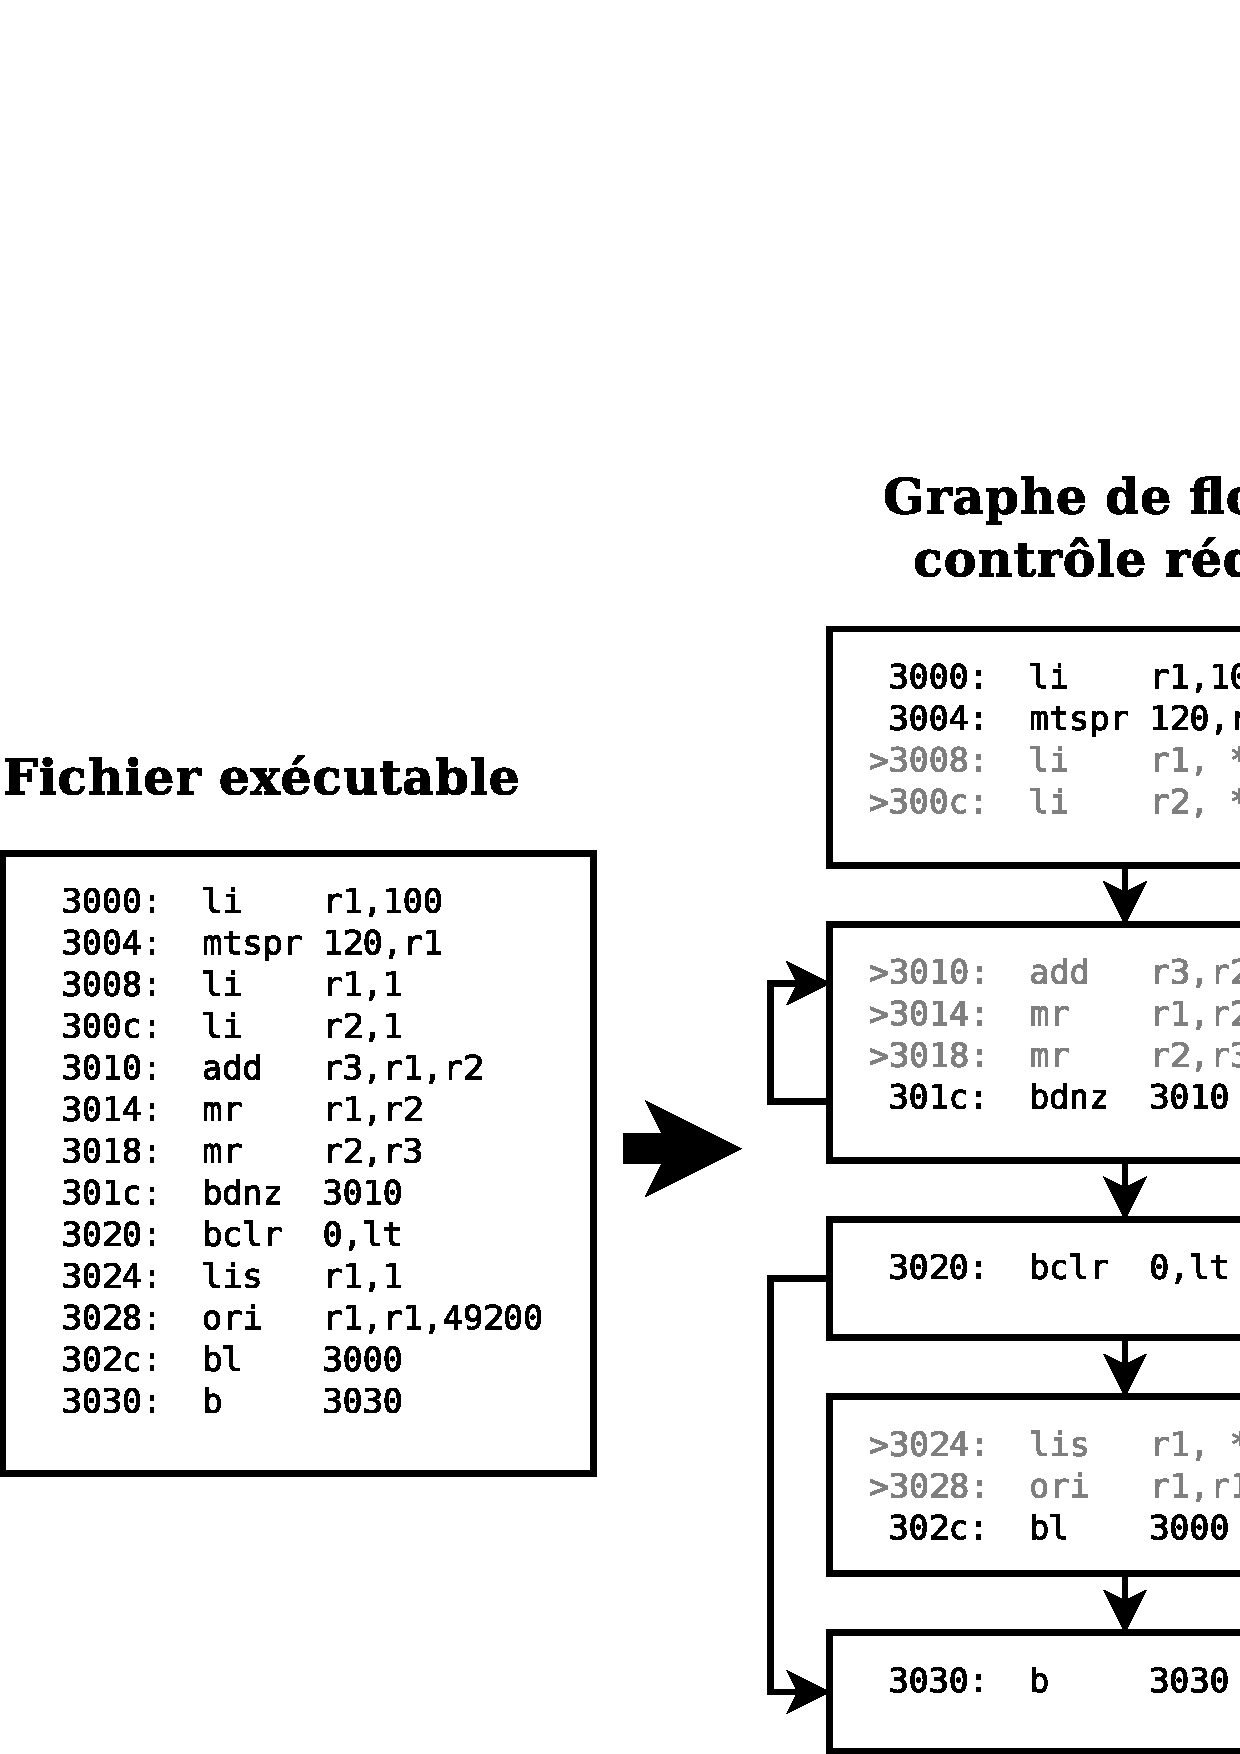
\includegraphics[scale=.4]{fig/cfg.pdf}
      \label{fig:cfg}}
    \hfill
    \subfloat[Simplified PDG of \texttt{fibcall-O2.elf}]{
      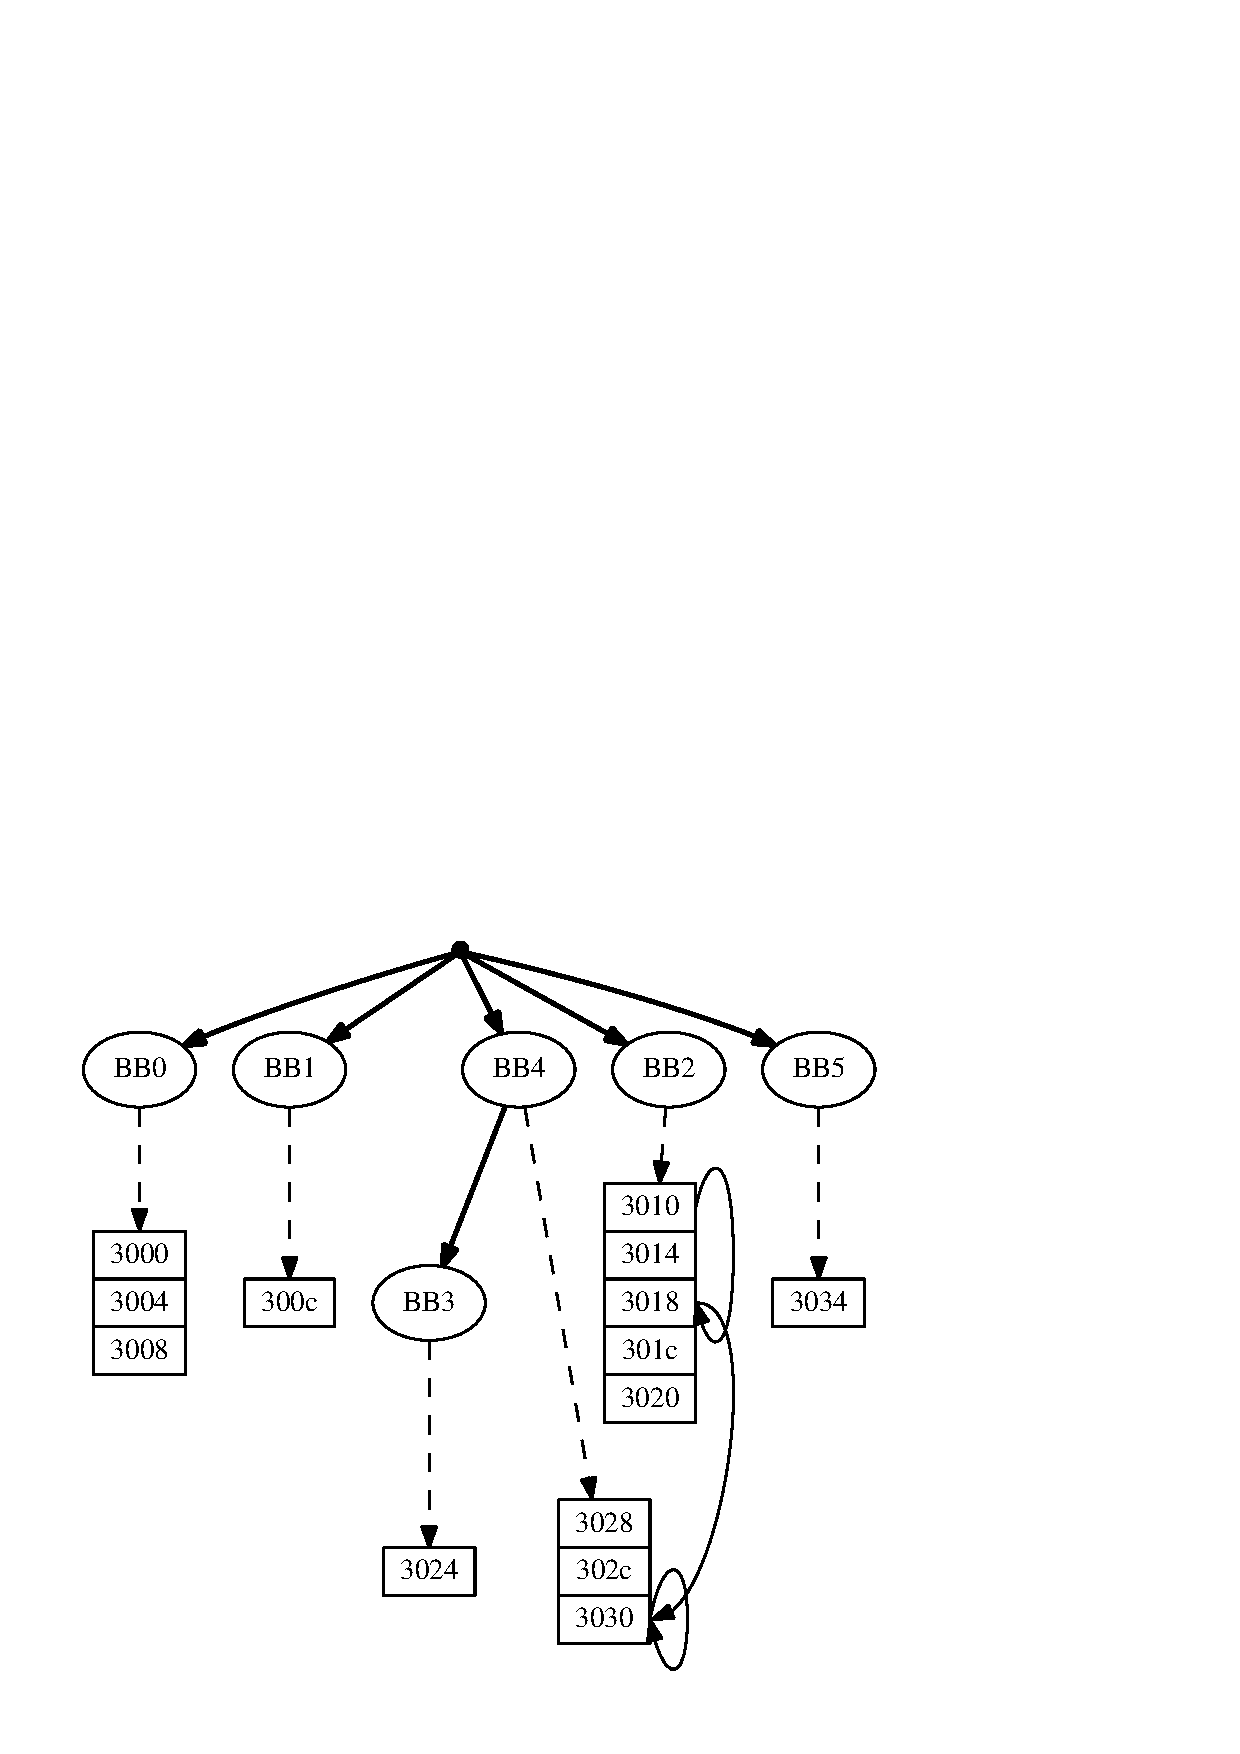
\includegraphics[scale=.4]{fig/pdg.pdf}
      \label{fig:pdg}}    \hspace{.5cm}

    \caption{CFG and PDG of a binary executable}
  \end{figure}

  In Figure~\ref{fig:pdg}, dashed, bold and solid edges represent respectively
  the belonging of a set of instructions to a block, a control dependency
  between two basic blocks, and a data dependency between two instructions.
  Considering once again the program in Figure~\ref{fig:dump} and the slicing
  criterion $\langle 3030, \{ctr\} \rangle$, we obtain the slice shown in
  Figure~\ref{fig:slice}. Indeed, the backward reachability analysis shows that
  the instruction at address $3030$ has a data dependency with the instruction
  at $3018$ which has also a data dependency with the instruction at $3010$ and
  the basic block $BB2$ has no control dependency apart from the entry point.

  Slicing the PDG is suboptimal for programs with procedure calls~\cite{KJL03}.
  %Moreover, inlining functions in the CFG does not scale.
  To overcome this limitation, inter-procedural slicing techniques use a
  fourth graph, the System Dependence Graph (SDG)~\cite{HSR90}. To build the
  SDG, in a first step, the PDG of each procedure must be built. In a second
  step, these PDGs are connected with call, parameter-in and parameter-out edges
  to account for procedure calls and parameters passing. The slicing algorithm
  on the SDG is based on two backwards analyses similar to the one used for the
  PDG. The first backward analysis does not follow parameters-out edges. It only
  adds to the slice instructions up to the entry point. The second backward
  analysis does not follow call and parameter-in edges. It adds to the slice all
  instructions down to the procedures output parameters. As a result, unwanted
  dependencies to output parameters from called procedures are not added to the
  slice.

  \subsection{Abstraction of programs for WCET estimation.}
  \label{subsec:slicing-reduction}
  
  Program slicing has many use cases in software engineering.
  In this paper we
  want to compute the set of memory locations that impact the WCET of a
  program. 
  To determine this set of locations we have to determine a suitable
  slicing criterion. This criterion is the set of pairs $\langle l,v\rangle$
  such that $l$ is the label of a conditional branch instruction and $v$ is the
  set of memory locations read by this instruction. If we consider the program
  in Figure~\ref{fig:dump}, it has only one conditional branch instruction:
  \verb|bdnz 3024| at address $3030$. The branch is taken if the count register
  $ctr$ is not zero. So, to compute the locations that should be part of the
  state of the model we have to compute the slice for the criteria $\{\langle
  3030, \{ctr\} \rangle\}$. The set of variables used either explicitly or
  implicitly by the initial program is $\{r1, r3, r8, r9, r10, lr, ctr\}$. The
  subset of variables used in the slice is $\{r8, ctr\}$ (see
  Figure~\ref{fig:slice}). Only these two registers have to be included in the
  state of the model.

  Let us underline that computing this slice gives us extra informations. For
  each register in the slice, we also know which instructions impact its value
  at a given execution point. In the general case, not all the instructions
  using a register in the slice are in the slice. Such instructions must be
  processed as instructions using registers not in the slice. Their output must
  not be written to the state. This allows to further reduce the number of
  states to explore.
  
